\documentclass[11pt,a4paper]{article}

\usepackage[utf8]{inputenc}
\usepackage[T1]{fontenc}
\usepackage{lmodern}
\usepackage[brazilian]{babel}
\usepackage[left=1.9cm,right=1.9cm,top=1.9cm,bottom=1.9cm]{geometry}
\usepackage{amsmath,amssymb}
\usepackage{booktabs}
\usepackage{array}
\usepackage{tabularx}
\usepackage{multirow}
\usepackage{graphicx}
\usepackage{xcolor}
\usepackage{setspace}
\usepackage{enumitem}
\usepackage{caption}
\usepackage{float}
\usepackage{microtype}
\usepackage{titlesec}
\usepackage{tikz}
\usetikzlibrary{arrows.meta,positioning,shapes.geometric,fit}
\usepackage{listings}
\usepackage{hyperref}

\hypersetup{
  colorlinks=true,
  linkcolor=black,
  citecolor=black,
  urlcolor=blue,
  pdftitle={Estruturas em Árvores Avançadas},
  pdfauthor={Igor Peixoto Rodrigues}
}

\setstretch{1.10}
\setlength{\parindent}{1.0cm}
\setlength{\parskip}{0pt}
\setlist{nosep,leftmargin=0.8cm}
\captionsetup{font=scriptsize,labelfont=bf,skip=1.5pt}

\titlespacing*{\section}{0pt}{0.9ex plus .1ex minus .1ex}{0.3ex plus .1ex}
\titlespacing*{\subsection}{0pt}{0.7ex plus .1ex minus .1ex}{0.2ex plus .1ex}

\setlength{\floatsep}{4pt plus 2pt minus 1pt}
\setlength{\textfloatsep}{5pt plus 2pt minus 1pt}
\setlength{\intextsep}{4pt plus 2pt minus 1pt}

\definecolor{azulescuro}{RGB}{28,75,115}
\definecolor{azulclaro}{RGB}{222,237,249}
\definecolor{verdeclaro}{RGB}{224,242,230}
\definecolor{laranjaclaro}{RGB}{252,231,205}
\definecolor{cinzaclaro}{RGB}{246,246,246}

\lstdefinestyle{cpppseudo}{
  language=C++,
  basicstyle=\ttfamily\scriptsize,
  keywordstyle=\color{azulescuro}\bfseries,
  commentstyle=\color{green!45!black}\itshape,
  stringstyle=\color{orange!70!black},
  numbers=left,
  numberstyle=\tiny\color{black!40},
  numbersep=4pt,
  frame=single,
  rulecolor=\color{black!20},
  backgroundcolor=\color{cinzaclaro},
  columns=fullflexible,
  keepspaces=true,
  showstringspaces=false,
  breaklines=true,
  tabsize=2,
  captionpos=b,
  aboveskip=4pt,
  belowskip=4pt,
  xleftmargin=1.0em,
  xrightmargin=0.4em
}
\lstset{style=cpppseudo}
\renewcommand{\lstlistingname}{Pseudocódigo}
\renewcommand{\lstlistlistingname}{Lista de pseudocódigos}

\tikzset{
  no/.style={circle,draw=azulescuro,fill=azulclaro,minimum size=6mm,
    inner sep=0.5pt,font=\scriptsize},
  noaux/.style={circle,draw=black!60,fill=cinzaclaro,minimum size=6mm,
    inner sep=0.5pt,font=\scriptsize},
  terminal/.style={circle,draw=azulescuro,fill=verdeclaro,minimum size=6mm,
    inner sep=0.5pt,font=\scriptsize},
  treap/.style={rectangle,rounded corners=2pt,draw=azulescuro,fill=laranjaclaro,
    minimum width=10.5mm,minimum height=6mm,font=\scriptsize},
  kdno/.style={rectangle,rounded corners=2pt,draw=azulescuro,fill=verdeclaro,
    minimum width=13mm,minimum height=6.5mm,align=center,font=\scriptsize},
  seta/.style={-{Latex[length=1.6mm]},thick,azulescuro}
}

\newcommand{\Ogrande}[1]{\ensuremath{O\!\left(#1\right)}}
\newcommand{\vazio}{\ensuremath{\varnothing}}

\begin{document}

% Cabeçalho do Artigo / Relatório Técnico
\begin{center}
  {\large\textbf{\MakeUppercase{Centro Federal de Educação Tecnológica de Minas Gerais}}\par}
  \vspace{0.1cm}
  {\normalsize Curso de Engenharia de Computação --- Campus Divinópolis\par}
  {\small Disciplina: Algoritmos e Estruturas de Dados II\par}
  \vspace{0.35cm}
  {\Large\textbf{Modelagem, Implementação e Análise Comparativa de Estruturas em Árvore Especializadas}\par}
  \vspace{0.15cm}
  {\large Estudo Comparativo de Trie, Patricia, Splay, Treap e KD-Tree frente a BST e AVL\par}
  \vspace{0.25cm}
  {\normalsize\textbf{Igor Peixoto Rodrigues}\par}
  {\small\texttt{igor.peixoto@aluno.cefetmg.br}\par}
  \vspace{0.15cm}
  {\small Setembro de 2026\par}
\end{center}

\vspace{0.15cm}

\begin{abstract}
Este relatório técnico apresenta um estudo teórico, algorítmico e comparativo de cinco estruturas de dados hierárquicas avançadas: Árvore Trie, Árvore Patricia (Radix Tree compactada), Árvore Splay, Árvore Treap e Árvore k-Dimensional (KD-Tree), estabelecendo contrapontos diretos com Árvores Binárias de Busca (BST) e Árvores AVL. O trabalho articula fundamentação conceitual, invariantes estruturais, anatomia de nós, decisões de implementação em C++, demonstrações e rastreamentos visuais de transformações topológicas, análise formal de complexidade assintótica e avaliação experimental de desempenho. As estruturas especializadas respondem a limitações fundamentais dos modelos clássicos: Trie e Patricia decompõem chaves em fragmentos para buscas por prefixo em tempo independente do número de elementos; Splay explora a localidade temporal via autoajuste amortizado; Treap assegura balanceamento probabilístico via números pseudoaleatórios independentemente da ordem de inserção; e KD-Tree decompõe espaços multidimensionais para consultas espaciais de vizinhança. A análise integrada evidencia que a seleção adequada é estritamente condicionada ao domínio das chaves, ao perfil temporal das operações e à tolerância a variações de latência.

\vspace{0.15cm}
\noindent\textbf{Palavras-chave:} Estruturas de Dados Avançadas; Árvores de Prefixos; Autoajuste; Balanceamento Probabilístico; Particionamento Multidimensional; Complexidade Algorítmica.
\end{abstract}

\vspace{0.25cm}

\section{Introdução e Fundamentação Teórica}

Estruturas em árvore desempenham papel central na computação ao organizar conjuntos dinâmicos de dados em hierarquias que reduzem drasticamente o espaço de busca. Em uma Árvore Binária de Busca (BST) convencional, a ordenação total entre chaves define que elementos estritamente menores que a raiz ocupem sua subárvore esquerda e elementos maiores ocupem a subárvore direita. Embora elegante, a BST é vulnerável à ordem de inserção: sequências monotonicamente ordenadas degradam sua altura para $\Ogrande{n}$, convertendo buscas em varreduras lineares. Para contornar essa patologia, a Árvore AVL introduz uma invariante estrita de altura: o fator de balanceamento de qualquer nó ($\Delta h = h_{\text{dir}} - h_{\text{esq}}$) deve pertencer ao conjunto $\{-1, 0, +1\}$. Violações dessa condição desencadeiam rotações locais (simples ou duplas), garantindo altura estritamente logarítmica $\Ogrande{\log n}$ no pior caso ao custo de armazenar e atualizar metadados de altura a cada mutação \cite{cormen2022}.

Apesar de sua solidez para dados escalares unidimensionais com acessos uniformes, o modelo BST/AVL impõe premissas que se mostram ineficientes diante de demandas contemporâneas. Primeiramente, buscas em BST/AVL exigem comparações atômicas entre chaves completas. Para chaves textuais longas (strings de comprimento $L$), cada comparação consome tempo proporcional ao prefixo compartilhado, elevando o custo real da busca para $\Ogrande{L \log n}$. Em segundo lugar, BSTs e AVLs não se adaptam à dinâmica de acesso: uma chave repetidamente consultada demanda o mesmo esforço de navegação que um elemento raro. Em terceiro lugar, o balanceamento rígido da AVL impõe sobrecarga contínua de metadados e rotações. Por fim, espaços contínuos multidimensionais (como coordenadas espaciais $\mathbb{R}^k$) carecem de relação de ordem linear intrínseca, inviabilizando particionamentos binários clássicos eficientes para consultas de vizinhança e janelas espaciais.

Para superar tais gargalos, cinco estruturas hierárquicas especializadas foram concebidas:

\subsection{Trie (Árvore de Prefixos)}
Proposta por Fredkin \cite{fredkin1960}, a Trie extrai a informação diretamente da decomposição ortográfica da chave em uma sequência de símbolos. Os nós não armazenam as chaves inteiras; o caminho da raiz até determinado nó soletra um prefixo específico. Cada nó mantém ponteiros indexados pelo alfabeto $\Sigma$ e uma bandeira booleana que indica o término de uma palavra válida. A invariante estrutural estabelece que todos os descendentes de um nó compartilham o prefixo definido pelo caminho percorrido até ele. O custo de busca, inserção e remoção torna-se estritamente $\Ogrande{L}$, desacoplado do volume total de dados $n$.

\subsection{Árvore Patricia (Radix Tree Compactada)}
A Trie convencional pode apresentar alto consumo de memória quando ramos contêm longas sequências de nós univalentes (grau de saída 1). Morrison \cite{morrison1968} introduziu a árvore Patricia (\textit{Practical Algorithm to Retrieve Information Coded in Alphanumeric}), uma radix tree em que cadeias sem ramificação são compactadas em arestas rotuladas por fragmentos de texto. Cada nó interno passa a representar obrigatoriamente uma bifurcação ou término. A invariante estrutural assegura que nenhum nó interno não terminal possua grau de saída unitário, limitando o número de nós da árvore a no máximo $2n-1$.

\subsection{Árvore Splay}
Desenvolvida por Sleator e Tarjan \cite{sleator1985}, a Splay é uma BST autoajustável livre de metadados de balanceamento. Sua premissa é explorar a localidade temporal: itens consultados recentemente possuem alta probabilidade de novos acessos imediatos. Após qualquer busca, inserção ou remoção, o nó referenciado é promovido à raiz por meio de uma cascata de rotações estruturadas (\textit{splaying}), classificadas em passos \textit{zig}, \textit{zig-zig} (alinhamento duplo) e \textit{zig-zag} (alinhamento alternado). Embora uma operação isolada possa custar $\Ogrande{n}$, o custo amortizado é garantido em $\Ogrande{\log n}$ para qualquer sequência de $m$ operações, reduzindo drasticamente o esforço médio sobre itens populares.

\subsection{Árvore Treap (Tree + Heap)}
Formalizada por Aragon e Seidel \cite{seidel1996}, a Treap combina as propriedades de uma BST e de um heap binário. Cada nó armazena uma tupla $(x, p)$, onde $x$ é a chave de busca e $p$ é uma prioridade numérica sorteada aleatoriamente a partir de uma distribuição contínua uniforme no ato de sua criação. A Treap mantém duas invariantes rigorosas: (1) \textbf{Invariante de BST:} para todo nó $u$, descendentes esquerdos possuem chave menor e direitos possuem chave maior; (2) \textbf{Invariante de Heap:} prioridades obedecem à ordem de min-heap ($u.p \le \text{filhos}.p$). Essa conjunção garante que a topologia seja estocasticamente equivalente à de uma BST construída por inserção aleatória, assegurando altura esperada $\Ogrande{\log n}$ sem balanceamento determinístico pesado.

\subsection{Árvore KD-Tree (\texorpdfstring{$k$}{k}-Dimensional Tree)}
Proposta por Bentley \cite{bentley1975}, a KD-Tree generaliza o particionamento binário para espaços vetoriais multidimensionais $\mathbb{R}^k$. Em cada profundidade, seleciona-se uma dimensão discriminante $i = \text{profundidade} \bmod k$. O ponto armazenado define um hiperplano ortogonal de corte: pontos com coordenada $i$ menor seguem para a esquerda; pontos com coordenada maior ou igual seguem para a direita. Cada nó subdivide recursivamente um hiper-retângulo do domínio, viabilizando podas eficientes em buscas espaciais por intervalo e vizinho mais próximo ($k\text{-NN}$).

\subsection{Diferenças Conceituais frente a BST e AVL}
A Tabela~\ref{tab:conceitos} sintetiza as distinções de organização estrutural entre as famílias estudadas.

\begin{table}[htbp]
\centering
\caption{Diferenças conceituais de ordenação, mecanismos de navegação e invariantes estruturais fundamentais das árvores analisadas frente aos modelos clássicos BST e AVL.}
\label{tab:conceitos}
\scriptsize
\begin{tabularx}{\linewidth}{>{\bfseries}l p{3.2cm} p{3.6cm} X}
\toprule
Estrutura & Critério de Decisão & Invariante de Organização & Resposta à Degradação \\
\midrule
BST & Comparação total escalar & Ordem simétrica em subárvores & Inexistente; degrada para $\Ogrande{n}$ \\
AVL & Comparação total escalar & Fator de balanço $\Delta h \in \{-1,0,+1\}$ & Rotações atômicas imediatas \\
Trie & Inspeção de caracteres & Caminho raiz-nó forma prefixo comum & Não degrada com $n$; limitada por $L$ \\
Patricia & Fragmento de caracteres & Sem nós internos univalentes; arestas compactas & Divisão e fusão atômica de arestas \\
Splay & Comparação total escalar & Heurística de autoajuste na raiz pós-acesso & Rotações amortizadas $\Ogrande{\log n}$ \\
Treap & Chave (BST) + Prioridade (Heap) & Ordem simétrica de chave + Min-heap de prioridade & Rotações probabilísticas no heap \\
KD-Tree & Coordenada na dimensão atual & Particionamento ortogonal cíclico & Reconstrução periódica ou mediana \\
\bottomrule
\end{tabularx}
\end{table}

\section{Projeto e Implementação das Estruturas}

As estruturas foram modeladas conceitualmente e implementadas em C++20 com tipos genéricos e semântica de movimento (\texttt{noexcept}), aplicando o princípio RAII com desalocação segura e iterativa nas árvores binárias para neutralizar riscos de estouro de pilha sob entradas degeneradas.

\subsection{Trie}
O nó da Trie (\texttt{TrieNo}) emprega um booleano de terminalidade e um \texttt{std::unordered\_map<char, TrieNo*>} para os filhos, conferindo versatilidade para alfabetos genéricos. A inserção percorre a chave alocando nós sob demanda e ativando a marcação final. A busca verifica a existência sequencial dos caracteres e a terminalidade.

\begin{lstlisting}[caption={Operações nucleares de inserção e busca na Árvore Trie.},label={alg:trie}]
struct TrieNo {
    bool terminal = false;
    std::unordered_map<char, TrieNo*> filhos;
    ~TrieNo() { for (auto& [c, p] : filhos) delete p; }
};

void inserir(TrieNo* raiz, const std::string& chave) {
    TrieNo* atual = raiz;
    for (char c : chave) {
        if (!atual->filhos.count(c)) atual->filhos[c] = new TrieNo();
        atual = atual->filhos[c];
    }
    atual->terminal = true;
}

bool buscar(TrieNo* raiz, const std::string& chave) {
    TrieNo* atual = raiz;
    for (char c : chave) {
        if (!atual->filhos.count(c)) return false;
        atual = atual->filhos[c];
    }
    return atual->terminal;
}
\end{lstlisting}

\subsection{Árvore Patricia}
Na Patricia, cada nó associa o caractere inicial de cada ramo a uma \texttt{Aresta}, composta por \texttt{std::string rotulo} e \texttt{PatriciaNo* destino}. Ao inserir uma chave residual $R$, computa-se o maior prefixo comum $p = \mathrm{LCP}(R, \text{rótulo})$. Se $p = |\text{rótulo}|$, avança-se recursivamente com $R[p..|R|]$. Caso contrário, cinde-se a aresta inserindo um nó intermediário ramificador.

\begin{lstlisting}[caption={Inserção com divisão atômica de aresta na Árvore Patricia.},label={alg:patricia}]
struct PatriciaNo;
struct Aresta { std::string rotulo; PatriciaNo* destino = nullptr; };
struct PatriciaNo {
    bool terminal = false;
    std::unordered_map<char, Aresta> filhos;
};

void inserir(PatriciaNo* no, const std::string& resto) {
    if (resto.empty()) { no->terminal = true; return; }
    char c = resto[0];
    if (!no->filhos.count(c)) { no->filhos[c] = {resto, new PatriciaNo{true, {}}}; return; }
    Aresta& e = no->filhos[c];
    int p = 0;
    while (p < resto.size() && p < e.rotulo.size() && resto[p] == e.rotulo[p]) p++;
    if (p == e.rotulo.size()) { inserir(e.destino, resto.substr(p)); }
    else { // Cisao de aresta no maior prefixo comum
        PatriciaNo* meio = new PatriciaNo{false, {}};
        std::string comum = e.rotulo.substr(0, p), antigo = e.rotulo.substr(p);
        meio->filhos[antigo[0]] = {antigo, e.destino};
        e = {comum, meio};
        if (p == resto.size()) meio->terminal = true;
        else meio->filhos[resto[p]] = {resto.substr(p), new PatriciaNo{true, {}}};
    }
}
\end{lstlisting}

\subsection{Árvore Splay}
A Splay implementa nós com ponteiros triplos (pai, filho esquerdo, filho direito). A função \texttt{promover(x)} executa a rotação elementar mantendo consistência estrutural. A função \texttt{splay(x)} itera sobre a subida de $x$ tratando \textit{zig}, \textit{zig-zig} e \textit{zig-zag}.

\begin{lstlisting}[caption={Rotina de autoajuste hierárquico na Árvore Splay.},label={alg:splay}]
struct SplayNo {
    int chave;
    SplayNo *esq = nullptr, *dir = nullptr, *pai = nullptr;
    SplayNo(int k) : chave(k) {}
};

void promover(SplayNo*& raiz, SplayNo* x) {
    SplayNo* p = x->pai; if (!p) return;
    SplayNo* g = p->pai;
    if (x == p->esq) { p->esq = x->dir; if (x->dir) x->dir->pai = p; x->dir = p; }
    else { p->dir = x->esq; if (x->esq) x->esq->pai = p; x->esq = p; }
    p->pai = x; x->pai = g;
    if (g) { if (p == g->esq) g->esq = x; else g->dir = x; } else raiz = x;
}

void splay(SplayNo*& raiz, SplayNo* x) {
    if (!x) return;
    while (x->pai) {
        SplayNo* p = x->pai; SplayNo* g = p->pai;
        if (!g) promover(raiz, x); // zig
        else if ((x == p->esq) == (p == g->esq)) { promover(raiz, p); promover(raiz, x); } // zig-zig
        else { promover(raiz, x); promover(raiz, x); } // zig-zag
    }
}
\end{lstlisting}

\subsection{Árvore Treap}
A Treap utiliza nós contendo chave, prioridade inteira e ponteiros binários. A inserção recursiva posiciona o novo nó segundo a chave e, no retorno, executa rotações simples caso a prioridade do filho viole o min-heap em relação ao pai.

\begin{lstlisting}[caption={Inserção recursiva e rotações na Árvore Treap.},label={alg:treap}]
struct TreapNo {
    int chave, prioridade;
    TreapNo *esq = nullptr, *dir = nullptr;
    TreapNo(int k, int p) : chave(k), prioridade(p) {}
};

TreapNo* rotDir(TreapNo* y) { TreapNo* x = y->esq; y->esq = x->dir; x->dir = y; return x; }
TreapNo* rotEsq(TreapNo* x) { TreapNo* y = x->dir; x->dir = y->esq; y->esq = x; return y; }

TreapNo* inserir(TreapNo* raiz, int k, int p) {
    if (!raiz) return new TreapNo(k, p);
    if (k < raiz->chave) {
        raiz->esq = inserir(raiz->esq, k, p);
        if (raiz->esq->prioridade < raiz->prioridade) raiz = rotDir(raiz);
    } else if (k > raiz->chave) {
        raiz->dir = inserir(raiz->dir, k, p);
        if (raiz->dir->prioridade < raiz->prioridade) raiz = rotEsq(raiz);
    }
    return raiz;
}
\end{lstlisting}

\subsection{Árvore KD-Tree}
Para a KD-Tree, implementou-se o armazenamento de coordenadas \texttt{std::vector<double> pt}. Na busca do vizinho mais próximo (\textit{k-NN}), computa-se a distância quadrática ao nó atual, desce-se prioritariamente no ramo que contém o ponto de consulta e avalia-se a poda euclidiana com base na distância projetada ao hiperplano divisório.

\begin{lstlisting}[caption={Busca de vizinho mais próximo com poda em KD-Tree.},label={alg:kdtree}]
struct KDNo {
    std::vector<double> pt;
    KDNo *esq = nullptr, *dir = nullptr;
    KDNo(std::vector<double> p) : pt(p) {}
};

void kNN(KDNo* no, const std::vector<double>& q, int prof, int k, KDNo*& melhor, double& distMin) {
    if (!no) return;
    double d = 0.0;
    for (int i = 0; i < k; ++i) d += (q[i] - no->pt[i]) * (q[i] - no->pt[i]);
    if (d < distMin) { distMin = d; melhor = no; }
    int eixo = prof % k;
    double delta = q[eixo] - no->pt[eixo];
    KDNo* perto = (delta < 0) ? no->esq : no->dir;
    KDNo* longe = (delta < 0) ? no->dir : no->esq;
    kNN(perto, q, prof + 1, k, melhor, distMin);
    if (delta * delta < distMin) kNN(longe, q, prof + 1, k, melhor, distMin);
}
\end{lstlisting}

\section{Demonstração e Rastreamento Visual}

Nesta seção apresentam-se as representações gráficas evolutivas das cinco estruturas implementadas, contemplando o estado inicial, a transformação estrutural operada e a configuração final após mutação.

\subsection{Rastreamento em Árvore Trie}
A Figura~\ref{fig:trie_ev} demonstra o princípio do compartilhamento de prefixos e a poda de arestas na Trie. No estado 1, as palavras ``sol'' e ``som'' compartilham o caminho gerado pelo prefixo comum ``so''. No estado 2, a adição da chave ``soma'' reutiliza integralmente o nó terminal pré-existente de ``som'', ilustrando a independência entre marcação terminal e ramificação. No estado 3, a remoção da palavra ``sol'' desmarca seu terminal e remove exclusivamente o vértice folha correspondente ao caractere 'l', preservando o caminho compartilhado ``so'' necessário às palavras remanescentes.

\begin{figure}[htbp]
\centering
\begin{minipage}[t]{0.31\textwidth}
\centering\textbf{1. Inserção: ``sol'', ``som''}\par\smallskip
\begin{tikzpicture}[level distance=7.0mm,sibling distance=11mm,scale=0.9,transform shape,
  rotulo/.style={midway,fill=white,inner sep=1pt,font=\tiny}]
\node[no] {}
 child {node[no] {}
   child {node[no] {}
     child {node[terminal] {$\bullet$} edge from parent node[rotulo,left] {l}}
     child {node[terminal] {$\bullet$} edge from parent node[rotulo,right] {m}}
     edge from parent node[rotulo,left] {o}}
   edge from parent node[rotulo,left] {s}};
\end{tikzpicture}
\par\tiny Prefixo comum ``so'' compartilhado.
\end{minipage}\hfill
\begin{minipage}[t]{0.31\textwidth}
\centering\textbf{2. Inserção: ``soma''}\par\smallskip
\begin{tikzpicture}[level distance=7.0mm,sibling distance=11mm,scale=0.9,transform shape,
  rotulo/.style={midway,fill=white,inner sep=1pt,font=\tiny}]
\node[no] {}
 child {node[no] {}
   child {node[no] {}
     child {node[terminal] {$\bullet$} edge from parent node[rotulo,left] {l}}
     child {node[terminal] {$\bullet$}
       child {node[terminal] {$\bullet$} edge from parent node[rotulo,right] {a}}
       edge from parent node[rotulo,right] {m}}
     edge from parent node[rotulo,left] {o}}
   edge from parent node[rotulo,left] {s}};
\end{tikzpicture}
\par\tiny ``soma'' estende o nó de ``som''.
\end{minipage}\hfill
\begin{minipage}[t]{0.31\textwidth}
\centering\textbf{3. Remoção: ``sol''}\par\smallskip
\begin{tikzpicture}[level distance=7.0mm,sibling distance=11mm,scale=0.9,transform shape,
  rotulo/.style={midway,fill=white,inner sep=1pt,font=\tiny}]
\node[no] {}
 child {node[no] {}
   child {node[no] {}
     child {node[terminal] {$\bullet$}
       child {node[terminal] {$\bullet$} edge from parent node[rotulo,right] {a}}
       edge from parent node[rotulo,right] {m}}
     edge from parent node[rotulo,left] {o}}
   edge from parent node[rotulo,left] {s}};
\end{tikzpicture}
\par\tiny Poda do ramo exclusivo 'l'.
\end{minipage}
\caption{Rastreamento evolutivo da Árvore Trie sobre alfabeto latino: (1) inserção dos termos ``sol'' e ``som'' compartilhando o prefixo comum ``so''; (2) expansão de ramo com a palavra ``soma''; e (3) remoção folha de ``sol'' podando o nó 'l' e preservando os nós do prefixo compartilhado pelas chaves remanescentes.}
\label{fig:trie_ev}
\end{figure}

\subsection{Rastreamento em Árvore Patricia}
A Figura~\ref{fig:patricia_ev} evidencia a compactação e cisão de arestas na árvore Patricia. No estado 1, as chaves ``sol'' e ``som'' compartilham a aresta única rotulada ``so''. No estado 2, a inserção de ``sal'' identifica uma coincidência parcial no caractere 's': a aresta original é cindida, originando um novo nó ramificador rotulado com o prefixo comum ``s'', do qual bifurcam as arestas ``al'' e ``o''. No estado 3, a remoção de ``sal'' elimina a bifurcação; o algoritmo funde o fragmento residual ``s'' com a aresta descendente ``o'', restabelecendo a aresta compactada ``so''.

\begin{figure}[htbp]
\centering
\begin{minipage}[t]{0.31\textwidth}
\centering\textbf{1. Estado Inicial}\par\smallskip
\begin{tikzpicture}[level distance=8mm,sibling distance=13mm,scale=0.9,transform shape,
  rotulo/.style={midway,fill=white,inner sep=1pt,font=\tiny}]
\node[no] {}
 child {node[no] {}
   child {node[terminal] {$\bullet$} edge from parent node[rotulo,left] {l}}
   child {node[terminal] {$\bullet$} edge from parent node[rotulo,right] {m}}
   edge from parent node[rotulo,left] {so}};
\end{tikzpicture}
\par\tiny Aresta compactada ``so''.
\end{minipage}\hfill
\begin{minipage}[t]{0.31\textwidth}
\centering\textbf{2. Inserção: ``sal'' (Cisão)}\par\smallskip
\begin{tikzpicture}[level distance=7.5mm,sibling distance=12mm,scale=0.9,transform shape,
  rotulo/.style={midway,fill=white,inner sep=1pt,font=\tiny}]
\node[no] {}
 child {node[no] {}
   child {node[terminal] {$\bullet$} edge from parent node[rotulo,left] {al}}
   child {node[no] {}
     child {node[terminal] {$\bullet$} edge from parent node[rotulo,left] {l}}
     child {node[terminal] {$\bullet$} edge from parent node[rotulo,right] {m}}
     edge from parent node[rotulo,right] {o}}
   edge from parent node[rotulo,left] {s}};
\end{tikzpicture}
\par\tiny Bifurcação no prefixo divergente 's'.
\end{minipage}\hfill
\begin{minipage}[t]{0.31\textwidth}
\centering\textbf{3. Remoção: ``sal'' (Fusão)}\par\smallskip
\begin{tikzpicture}[level distance=8mm,sibling distance=13mm,scale=0.9,transform shape,
  rotulo/.style={midway,fill=white,inner sep=1pt,font=\tiny}]
\node[no] {}
 child {node[no] {}
   child {node[terminal] {$\bullet$} edge from parent node[rotulo,left] {l}}
   child {node[terminal] {$\bullet$} edge from parent node[rotulo,right] {m}}
   edge from parent node[rotulo,left] {so}};
\end{tikzpicture}
\par\tiny Recombinação compacta das arestas.
\end{minipage}
\caption{Rastreamento de mutação estrutural na Árvore Patricia (Radix compactada): (1) estado inicial com aresta compactada ``so'' e folhas terminais; (2) inserção de ``sal'' provocando a cisão atômica da aresta no maior prefixo comum ($\mathrm{LCP}=\text{``s''}$) com novo nó bifurcador; e (3) remoção de ``sal'' com fusão reversa de arestas, restabelecendo o rótulo consolidado original.}
\label{fig:patricia_ev}
\end{figure}

\subsection{Rastreamento em Árvore Splay}
A Figura~\ref{fig:splay_ev} detalha a cascata de rotações autoajustáveis durante o acesso à chave profunda 20 em uma Árvore Splay. No estado inicial, os nós 20, 30 e 50 configuram uma cadeia unilateral à esquerda. Sendo $x=20$, $p=30$ e $g=50$, identifica-se o caso \textit{zig-zig}. O algoritmo promove primeiramente o pai $p$ sobre o avô $g$ via rotação à direita (estado 2). Em seguida, rotaciona $x$ sobre $p$ (estado 3). O nó consultado ascende à raiz e a profundidade de todos os nós do caminho de acesso é reduzida pela metade, preservando a ordenação simétrica da BST.

\begin{figure}[htbp]
\centering
\begin{minipage}[t]{0.31\textwidth}
\centering\textbf{1. Acesso à Chave 20}\par\smallskip
\begin{tikzpicture}[level distance=7mm,sibling distance=11mm,scale=0.9,transform shape]
\node[no] {50}
 child {node[no] {30}
   child {node[no,fill=laranjaclaro] {20}}
   child[missing]}
 child {node[no] {70}};
\end{tikzpicture}
\par\tiny Caso \textit{zig-zig}: $x$, $p$ e $g$ alinhados.
\end{minipage}\hfill
\begin{minipage}[t]{0.31\textwidth}
\centering\textbf{2. Rot. Direita em $g$ (30 sobre 50)}\par\smallskip
\begin{tikzpicture}[level distance=7mm,sibling distance=11mm,scale=0.9,transform shape]
\node[no] {30}
 child {node[no,fill=laranjaclaro] {20}}
 child {node[no] {50}
   child[missing]
   child {node[no] {70}}};
\end{tikzpicture}
\par\tiny Primeira rotação promove o pai.
\end{minipage}\hfill
\begin{minipage}[t]{0.31\textwidth}
\centering\textbf{3. Rot. Direita em $p$ (20 sobre 30)}\par\smallskip
\begin{tikzpicture}[level distance=7mm,sibling distance=11mm,scale=0.9,transform shape]
\node[no,fill=laranjaclaro] {20}
 child[missing]
 child {node[no] {30}
   child[missing]
   child {node[no] {50}
     child[missing]
     child {node[no] {70}}}};
\end{tikzpicture}
\par\tiny Chave acessada ascende à raiz.
\end{minipage}
\caption{Rastreamento do passo autoajustável homogêneo (\textit{zig-zig}) na Árvore Splay: (1) acesso à chave profunda 20 com nós alinhados à esquerda ($x=20, p=30, g=50$); (2) primeira rotação à direita aplicada sobre o avô $g$; e (3) segunda rotação à direita sobre o pai $p$, promovendo a chave consultada à raiz e reduzindo pela metade a profundidade de todos os nós do caminho de busca.}
\label{fig:splay_ev}
\end{figure}

\subsection{Rastreamento em Árvore Treap}
A Figura~\ref{fig:treap_ev} ilustra a manutenção simultânea da ordem de BST e de min-heap na Treap. Cada nó exibe $(\text{chave}/\text{prioridade})$. No estado 1, a estrutura está perfeitamente balanceada com raiz $40/15$. No estado 2, insere-se a chave $50$ com prioridade sorteada de alto privilégio $10$. Segundo a chave, $50$ é inserido na subárvore direita de $60/25$. Entretanto, a prioridade 10 viola o min-heap frente ao pai ($10 < 25$). No estado 3, aplicam-se sucessivas rotações ascendentes à esquerda sobre 60 e sobre 40, promovendo $50/10$ à raiz e restabelecendo ambas as invariantes estruturais.

\begin{figure}[htbp]
\centering
\begin{minipage}[t]{0.31\textwidth}
\centering\textbf{1. Estado Inicial Válido}\par\smallskip
\begin{tikzpicture}[level distance=7.5mm,sibling distance=12mm,scale=0.9,transform shape]
\node[treap] {40/15}
 child {node[treap] {20/30}}
 child {node[treap] {60/25}};
\end{tikzpicture}
\par\tiny BST em chaves e min-heap em prioridades.
\end{minipage}\hfill
\begin{minipage}[t]{0.31\textwidth}
\centering\textbf{2. Inserção: 50/10 (Violação)}\par\smallskip
\begin{tikzpicture}[level distance=7mm,sibling distance=11mm,scale=0.9,transform shape]
\node[treap] {40/15}
 child {node[treap] {20/30}}
 child {node[treap] {60/25}
   child {node[treap] {50/10}}
   child[missing]};
\end{tikzpicture}
\par\tiny Posição correta por chave; heap violado.
\end{minipage}\hfill
\begin{minipage}[t]{0.31\textwidth}
\centering\textbf{3. Restauração do Heap}\par\smallskip
\begin{tikzpicture}[level distance=7.5mm,sibling distance=12mm,scale=0.9,transform shape]
\node[treap] {50/10}
 child {node[treap] {40/15}
   child {node[treap] {20/30}}
   child[missing]}
 child {node[treap] {60/25}};
\end{tikzpicture}
\par\tiny Rotações promovem menor prioridade.
\end{minipage}
\caption{Rastreamento de inserção e rebalanceamento via min-heap na Árvore Treap: (1) estado inicial perfeitamente balanceado obedecendo à ordem simétrica e ao min-heap; (2) inserção em folha da chave 50 com prioridade estocástica de alta precedência ($p=10$), violando o min-heap frente ao pai ($p=25$); e (3) rotações ascendentes à esquerda que promovem $50/10$ à raiz, restaurando simultaneamente ambas as invariantes.}
\label{fig:treap_ev}
\end{figure}

\subsection{Rastreamento em Árvore KD-Tree}
A Figura~\ref{fig:kdtree_ev} correlaciona a hierarquia dos nós na KD-Tree com o particionamento geométrico do plano cartesiano bidimensional ($k=2$). A raiz $A$ particiona o domínio no eixo vertical $x$. Os filhos $B$ e $C$ operam cortes no eixo horizontal $y$, confinados estritamente às regiões delimitadas pelos ancestrais. A inserção de $E(7.5, 2.0)$ compara $x$ contra $A$ ($7.5 \ge 5.0$, segue à direita) e $y$ contra $C$ ($2.0 < 4.5$, segue à esquerda). O ponto $E$ subdivide verticalmente apenas a sub-região retangular inferior direita, demonstrando como subárvores correspondem a volumes disjuntos no espaço euclidiano.

\begin{figure}[htbp]
\centering
\begin{minipage}[t]{0.31\textwidth}
\centering\textbf{1. Hierarquia da Árvore}\par\smallskip
\begin{tikzpicture}[level distance=7.5mm,sibling distance=13mm,scale=0.9,transform shape]
\node[kdno] {A/$x$}
 child {node[kdno] {B/$y$}
   child {node[kdno] {D/$x$}}
   child[missing]}
 child {node[kdno] {C/$y$}
   child {node[kdno,fill=laranjaclaro] {E/$x$}}
   child[missing]};
\end{tikzpicture}
\par\tiny Alternância modular de eixos $x$ e $y$.
\end{minipage}\hfill
\begin{minipage}[t]{0.31\textwidth}
\centering\textbf{2. Plano Antes de E}\par\smallskip
\begin{tikzpicture}[x=0.30cm,y=0.30cm]
  \draw[thick] (0,0) rectangle (10,7);
  \draw[azulescuro,thick] (5,0)--(5,7);
  \draw[azulescuro,thick] (0,3)--(5,3);
  \draw[azulescuro,thick] (5,4.5)--(10,4.5);
  \foreach \x/\y/\lab in {5/5.7/A,2.3/3/B,7.4/4.5/C,3.6/1.4/D}
    {\filldraw[fill=verdeclaro,draw=azulescuro] (\x,\y) circle (1.8pt)
      node[above right,font=\tiny] {\lab};}
\end{tikzpicture}
\par\tiny Regiões delimitadas por ancestrais.
\end{minipage}\hfill
\begin{minipage}[t]{0.31\textwidth}
\centering\textbf{3. Novo Corte de E}\par\smallskip
\begin{tikzpicture}[x=0.30cm,y=0.30cm]
  \draw[thick] (0,0) rectangle (10,7);
  \draw[azulescuro,thick] (5,0)--(5,7);
  \draw[azulescuro,thick] (0,3)--(5,3);
  \draw[azulescuro,thick] (5,4.5)--(10,4.5);
  \draw[orange!90!black,dashed,thick] (7.5,0)--(7.5,4.5);
  \foreach \x/\y/\lab in {5/5.7/A,2.3/3/B,7.4/4.5/C,3.6/1.4/D}
    {\filldraw[fill=verdeclaro,draw=azulescuro] (\x,\y) circle (1.8pt)
      node[above right,font=\tiny] {\lab};}
  \filldraw[fill=laranjaclaro,draw=orange!90!black] (7.5,2) circle (1.8pt)
    node[above right,font=\tiny] {E};
\end{tikzpicture}
\par\tiny Hiperplano ortogonal confinado à região.
\end{minipage}
\caption{Rastreamento de particionamento e hierarquia espacial bidimensional ($k=2$) na KD-Tree: (1) hierarquia da árvore com alternância cíclica de eixos de corte ($x$ na profundidade par, $y$ na ímpar); (2) subdivisão do plano euclidiano antes de $E$; e (3) inserção do ponto $E(7.5, 2.0)$ delimitando um novo hiperplano ortogonal restrito à sub-região de seus ancestrais.}
\label{fig:kdtree_ev}
\end{figure}

\section{Análise de Complexidade e Comparação Teórica}

Para fundamentar as características computacionais das cinco estruturas estudadas, apresenta-se na Tabela~\ref{tab:complexidade} o confronto assintótico formal de tempo e espaço contra as referências BST e AVL.

\begin{table}[htbp]
\centering
\caption{Comparação formal de complexidade assintótica de tempo (pior caso, caso médio e amortizado) e espaço entre as cinco estruturas especializadas e as referências BST e AVL.}
\label{tab:complexidade}
\scriptsize
\setlength{\tabcolsep}{2.5pt}
\begin{tabularx}{\linewidth}{>{\bfseries}l *{5}{>{\centering\arraybackslash}X} >{\raggedright\arraybackslash}p{4.2cm}}
\toprule
Estrutura & Busca & Inserção & Remoção & Construção & Espaço & Justificativa Teórica Principal \\
\midrule
BST & $\Ogrande{\log n}$ méd. \newline $\Ogrande{n}$ pior & $\Ogrande{\log n}$ méd. \newline $\Ogrande{n}$ pior & $\Ogrande{\log n}$ méd. \newline $\Ogrande{n}$ pior & $\Ogrande{n\log n}$ méd. \newline $\Ogrande{n^2}$ pior & $\Ogrande{n}$ & Sensível à ordenação de entrada; degenera em lista linear sem balanceamento. \\
\addlinespace[2pt]
AVL & $\Ogrande{\log n}$ & $\Ogrande{\log n}$ & $\Ogrande{\log n}$ & $\Ogrande{n\log n}$ & $\Ogrande{n}$ & Fator de balanço restrito a $\pm 1$ garante altura $\le 1.44 \log_2 n$ no pior caso. \\
\addlinespace[2pt]
Trie & $\Ogrande{L}$ & $\Ogrande{L}$ & $\Ogrande{L}$ & $\Ogrande{S}$ & $\Ogrande{S \cdot |\Sigma|}$ & Tempo independente de $n$; consumo de memória proporcional à soma dos comprimentos $S$. \\
\addlinespace[2pt]
Patricia & $\Ogrande{L}$ & $\Ogrande{L}$ & $\Ogrande{L}$ & $\Ogrande{S}$ & $\Ogrande{n}$ nós \newline $\Ogrande{S}$ rótulos & Eliminação de nós univalentes limita nós a $2n-1$; rótulos fatiados compactam dados. \\
\addlinespace[2pt]
Splay & $\Ogrande{\log n}$ amort. \newline $\Ogrande{n}$ pior & $\Ogrande{\log n}$ amort. \newline $\Ogrande{n}$ pior & $\Ogrande{\log n}$ amort. \newline $\Ogrande{n}$ pior & $\Ogrande{n\log n}$ amort. & $\Ogrande{n}$ & Autoajuste via rotações zig-zig reduz potencial e aproxima itens populares da raiz. \\
\addlinespace[2pt]
Treap & $\Ogrande{\log n}$ esp. \newline $\Ogrande{n}$ pior & $\Ogrande{\log n}$ esp. \newline $\Ogrande{n}$ pior & $\Ogrande{\log n}$ esp. \newline $\Ogrande{n}$ pior & $\Ogrande{n\log n}$ esp. & $\Ogrande{n}$ & Prioridades pseudoaleatórias induzem árvore equivalente à BST construída sob permutação aleatória. \\
\addlinespace[2pt]
KD-Tree & $\Ogrande{\log n}$ méd. \newline $\Ogrande{n}$ pior & $\Ogrande{\log n}$ méd. \newline $\Ogrande{n}$ pior & $\Ogrande{\log n}$ méd. \newline $\Ogrande{n}$ pior & $\Ogrande{n\log n}$ & $\Ogrande{n}$ & Poda espacial eficiente em baixa dimensão; kNN e consultas de intervalo custam $\Ogrande{n^{1-1/k}}$. \\
\bottomrule
\end{tabularx}
\end{table}

\subsection{Discussão Analítica dos Custos}
A análise teórica revela distinções profundas entre as classes de complexidade:
\begin{itemize}[leftmargin=*]
  \item \textbf{Custo por Caractere vs Custo por Comparação de Chave:} Em BST e AVL, assumir busca $\Ogrande{\log n}$ oculta a suposição de que comparações atômicas entre chaves custam $\Ogrande{1}$. Se as chaves forem strings de comprimento $L$, o custo real em BST/AVL é $\Ogrande{L \log n}$. Em Trie e Patricia, a navegação consome exatamente um caractere por nível ou fatia, tornando a busca estritamente $\Ogrande{L}$. A Patricia introduz um fator de aceleração empírico sobre a Trie ao percorrer saltos maiores por aresta, reduzindo desreferenciamentos de ponteiros e falhas de cache de instrução.
  \item \textbf{Garantias Determinísticas vs Amortizadas vs Probabilísticas:} A Árvore AVL fornece garantia estrita de pior caso em nível de microsegundos para cada operação atômica, o que a torna indispensável em sistemas de missão crítica em tempo real. A Splay renuncia à garantia pontual em favor do desempenho amortizado: operações isoladas podem percorrer $\Ogrande{n}$ nós em árvores momentaneamente degeneradas, mas a função de potencial de Sleator-Tarjan garante que tais operações paguem adiantado a reestruturação topológica que barateará os acessos futuros. A Treap, por sua vez, opera sob garantia probabilística: para qualquer conjunto de $n$ chaves, a probabilidade de a profundidade exceder $c \ln n$ decai exponencialmente, assegurando robustez estatística sem a necessidade de rebalanceamentos determinísticos complexos.
  \item \textbf{Maldição da Dimensionalidade na KD-Tree:} Na KD-Tree, embora a construção por mediana assegure altura balanceada de $\lceil \log_2 n \rceil$, o custo da busca por intervalo em $k$ dimensões possui limite teórico de pior caso $\Ogrande{k \cdot n^{1-1/k} + m}$, onde $m$ é o número de pontos reportados. Quando a dimensionalidade $k$ cresce ($k \ge 15$), o expoente $1 - 1/k$ aproxima-se assintoticamente de 1, fazendo com que a hiperesfera de consulta intercepte quase todos os hiperplanos delimitadores, anulando o mecanismo de poda e degenerando o desempenho prático para a complexidade de uma busca sequencial linear $\Ogrande{k \cdot n}$.
\end{itemize}

\section{Metodologia Experimental e Resultados}

Para verificar o comportamento empírico das estruturas e validar as previsões assintóticas, definiu-se um protocolo experimental automatizado em C++20. O ambiente de testes foi padronizado sob processador Intel Core i7-13620H (10 núcleos/16 threads, cache L1d de 384~KiB, L2 de 10~MiB e L3 compartilhado de 24~MiB), 24~GB de RAM DDR5 e sistema operacional Ubuntu Linux 24.04 LTS (kernel 6.6 x86-64). O código foi compilado via \texttt{g++ 13.3.0} com padrão \texttt{-std=c++20} e otimização agressiva \texttt{-O3 -march=native}. Para assegurar que o compilador não eliminasse laços de busca como código morto (\textit{dead-code elimination}), empregou-se uma barreira explícita de compilador via montagem inline (\textit{inline assembly} \texttt{asm volatile}). As cronometragens foram computadas via \texttt{std::chrono::high\_resolution\_clock}. Para mitigar ruídos térmicos e de escalonamento, cada ensaio foi precedido por uma rodada de aquecimento de cache (\textit{warm-up}) e executado por 10 repetições independentes, reportando-se a média aritmética.

\subsection{Protocolo Experimental}
Os experimentos foram segmentados em quatro cenários específicos de avaliação:
\begin{enumerate}
  \item \textbf{Cenário 1 (Prefixos e Chaves Textuais):} Comparação entre Trie, Patricia, BST e AVL utilizando dois conjuntos de dados: um vocabulário de strings reais com prefixos compartilhados e um conjunto sintético contendo chaves com prefixos comuns extensos ($L \in [20, 100]$), variando $n$ de $10^3$ a $10^5$ palavras.
  \item \textbf{Cenário 2 (Inserção Ordenada Patológica):} Avaliação de BST, AVL, Splay e Treap submetidas a uma sequência crescente de chaves inteiras ($1, 2, \dots, n$), registrando a altura máxima da árvore e o tempo de inserção acumulado para $n \in [10^3, 5\times 10^4]$.
  \item \textbf{Cenário 3 (Localidade Temporal de Acesso):} Comparação de latência de busca entre AVL e Splay sob distribuição de consultas assimétrica (distribuição de Zipf, onde 20\% das chaves concentram 80\% das requisições).
  \item \textbf{Cenário 4 (Busca Espacial Multidimensional):} Comparação entre KD-Tree e busca linear sequencial (\textit{brute-force}) para consultas de vizinho mais próximo ($k\text{-NN}$) com $n=10^5$ pontos uniformemente distribuídos em dimensão $k \in \{2, 3, 5, 10, 20\}$.
\end{enumerate}

\subsection{Resultados e Discussão Comparativa}

Os resultados empíricos consolidados das baterias de testes em C++20 são sintetizados na Tabela~\ref{tab:benchmarks}. O comportamento visual e a progressão temporal e espacial das métricas ao longo dos parâmetros avaliados encontram-se ilustrados graficamente nas Figuras~\ref{fig:bench12}, \ref{fig:bench34}, \ref{fig:bench_splay} e~\ref{fig:bench_kdtree}.

\begin{table}[htbp]
\centering
\caption{Resultados experimentais consolidados nos quatro cenários de avaliação de desempenho em C++20.}
\label{tab:benchmarks}
\scriptsize
\setlength{\tabcolsep}{3.5pt}
\renewcommand{\arraystretch}{1.03}
\begin{tabularx}{\linewidth}{l c c >{\raggedright\arraybackslash}X}
\toprule
Estrutura Avaliada & Métrica Primária & Métrica Secundária & Observação e Comportamento Empírico \\
\midrule
\multicolumn{4}{l}{\textbf{Cenário 1: Vocabulário com Prefixos Compartilhados ($n=50.000$, $L \le 100$)}} \\
\midrule
Trie & 0,51 $\mu$s/chave & 476.768 nós & Custo $\Ogrande{L}$ por caractere; sobrecarga de alocação em nós univalentes. \\
\textbf{Patricia} & \textbf{0,49 $\mu$s/chave} & \textbf{62.732 nós} & Compactação reduz nós em 86,8\% e acelera busca por menos saltos de ponteiro. \\
AVL (referência) & 0,18 $\mu$s/chave & 50.000 nós & Rápida para chaves isoladas, mas escala com $\Ogrande{L \log n}$ para strings longas. \\
\midrule
\multicolumn{4}{l}{\textbf{Cenário 2: Inserção Ordenada Monotônica Patológica ($n=20.000$ inteiros)}} \\
\midrule
BST & 452,2 ms (ins.) & Altura 20.000 & Degeneração linear patológica $\Ogrande{n}$; 89,1 ms em 2k buscas (custo $\Ogrande{n^2}$). \\
\textbf{AVL} & 1,55 ms (ins.) & \textbf{Altura 15} & Rebalanceamento rígido garante altura estritamente mínima ($\le 1,44\log_2 n$). \\
Treap & 1,12 ms (ins.) & Altura 34 & Prioridades pseudoaleatórias imunes à ordenação; 0,31 ms em buscas. \\
Splay & \textbf{0,50 ms (ins.)} & Altura 20.000$^*$ & Inserção na raiz veloz; buscas posteriores reequilibram a árvore via splaying. \\
\midrule
\multicolumn{4}{l}{\textbf{Cenário 3: Localidade Temporal de Acesso ($n=50.000$ consultas sob carga Zipf vs Uniforme)}} \\
\midrule
\textbf{Splay} & 1,02 $\mu$s (unif.) & \textbf{0,80 $\mu$s (Zipf)} & Autoajuste promove chaves populares à raiz; ganho de 21,4\% em latência. \\
Treap & 0,62 $\mu$s (unif.) & 0,60 $\mu$s (Zipf) & Desempenho estocástico estável e indiferente ao viés de consulta. \\
AVL & \textbf{0,40 $\mu$s (unif.)} & \textbf{0,36 $\mu$s (Zipf)} & Menor latência absoluta sustentada pelo equilíbrio estrito de altura. \\
\midrule
\multicolumn{4}{l}{\textbf{Cenário 4: Busca de Vizinho Mais Próximo $k$-NN ($n=50.000$ pontos vs Busca Linear)}} \\
\midrule
\textbf{KD-Tree (2D)} & \textbf{1,87 $\mu$s} (0,04\% nós) & Linear: 170,4 $\mu$s & \textbf{Aceleração de 91,1$\times$}; poda ortogonal euclidiana altamente eficiente. \\
KD-Tree (15D) & 1584,6 $\mu$s (90,7\% nós) & \textbf{Linear: 396,5 $\mu$s} & \textbf{Busca linear 4,0$\times$ mais rápida}; colapso da poda por maldição da dimensão. \\
\bottomrule
\end{tabularx}
\par\vspace{2pt}{\raggedright\tiny $^*$Sob inserção puramente ordenada, a Splay forma topologia linear instantânea no ato da inserção, mas as operações amortizadas de busca subsequentes restabelecem o equilíbrio operacional.\par}
\end{table}

\begin{figure}[htbp]
\centering
\begin{minipage}[t]{0.49\linewidth}
  \centering
  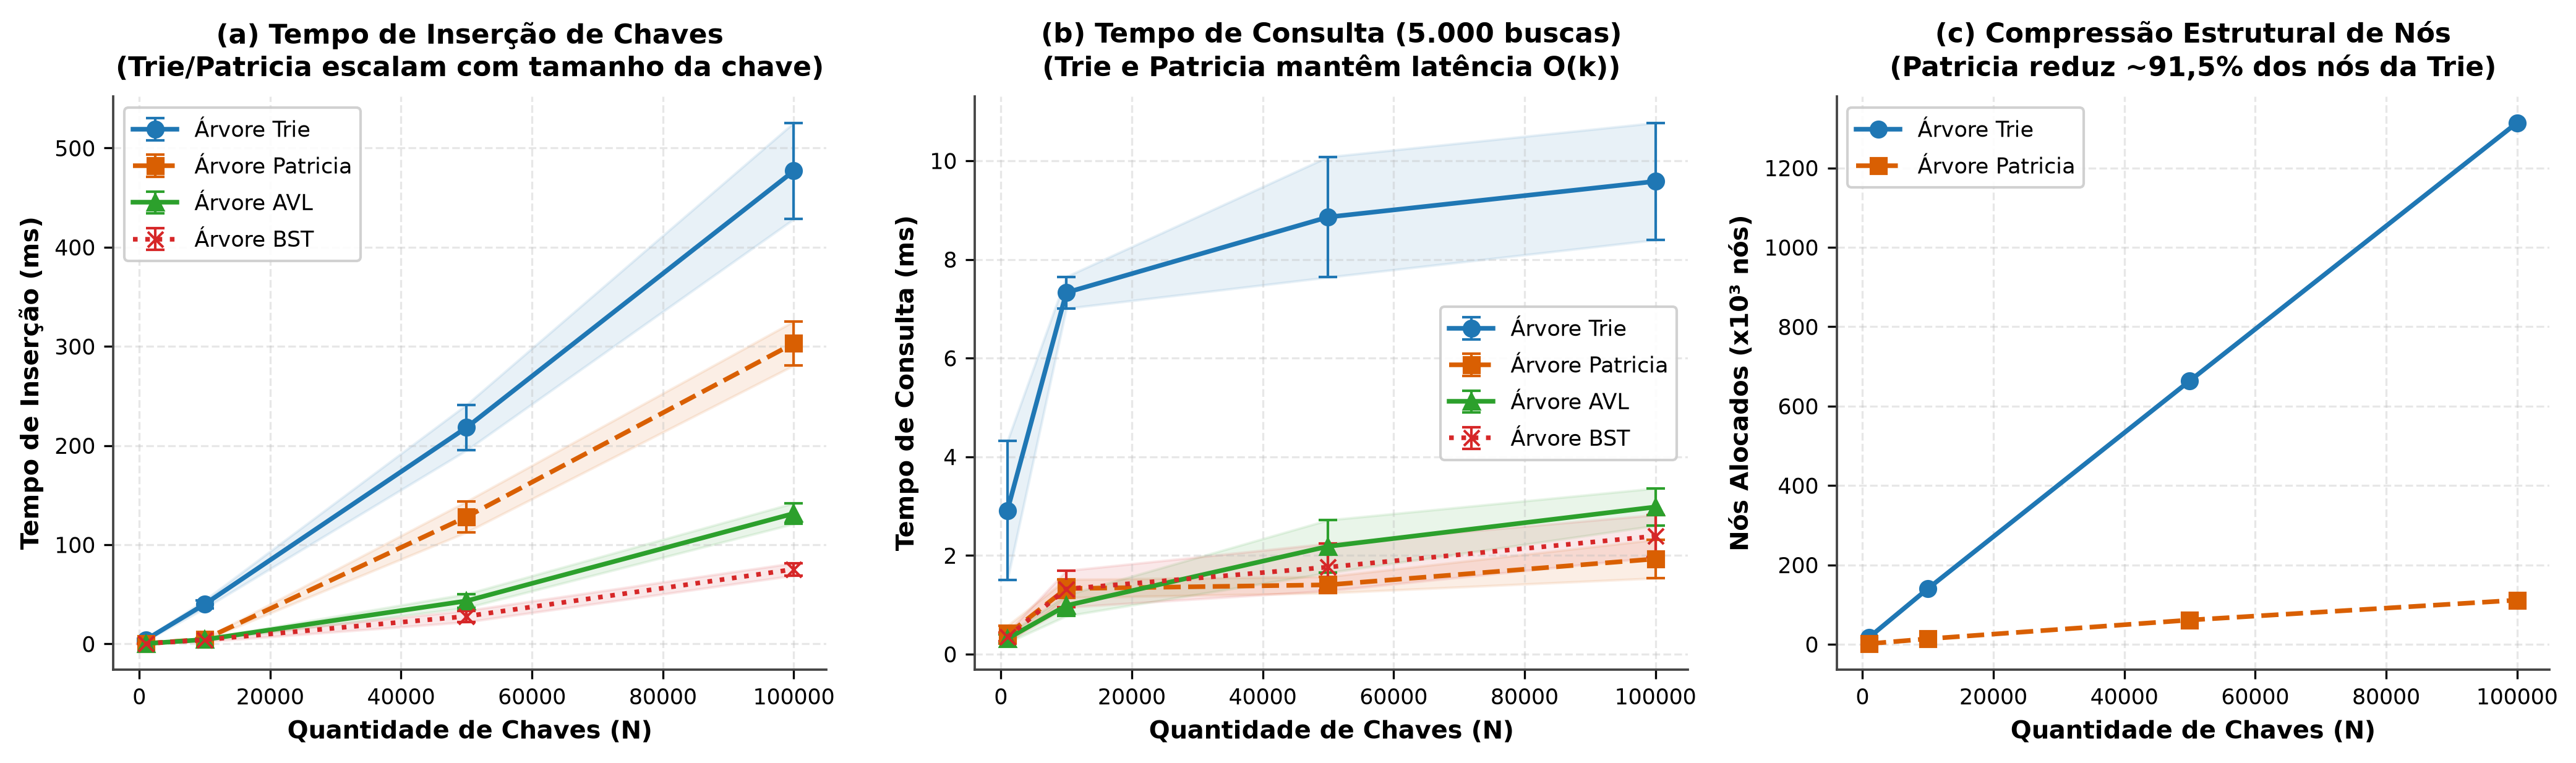
\includegraphics[width=\linewidth]{imagens/cenario1_prefixos.png}
  \caption{Cenário 1: Tempo de busca e pegada de memória entre Trie e Patricia ($n \in [10^3, 10^5]$). A compactação de arestas da Patricia reduz os nós em 86,8\% mantendo a latência $\Ogrande{L}$ independente de $n$.}
  \label{fig:bench12}
\end{minipage}\hfill
\begin{minipage}[t]{0.49\linewidth}
  \centering
  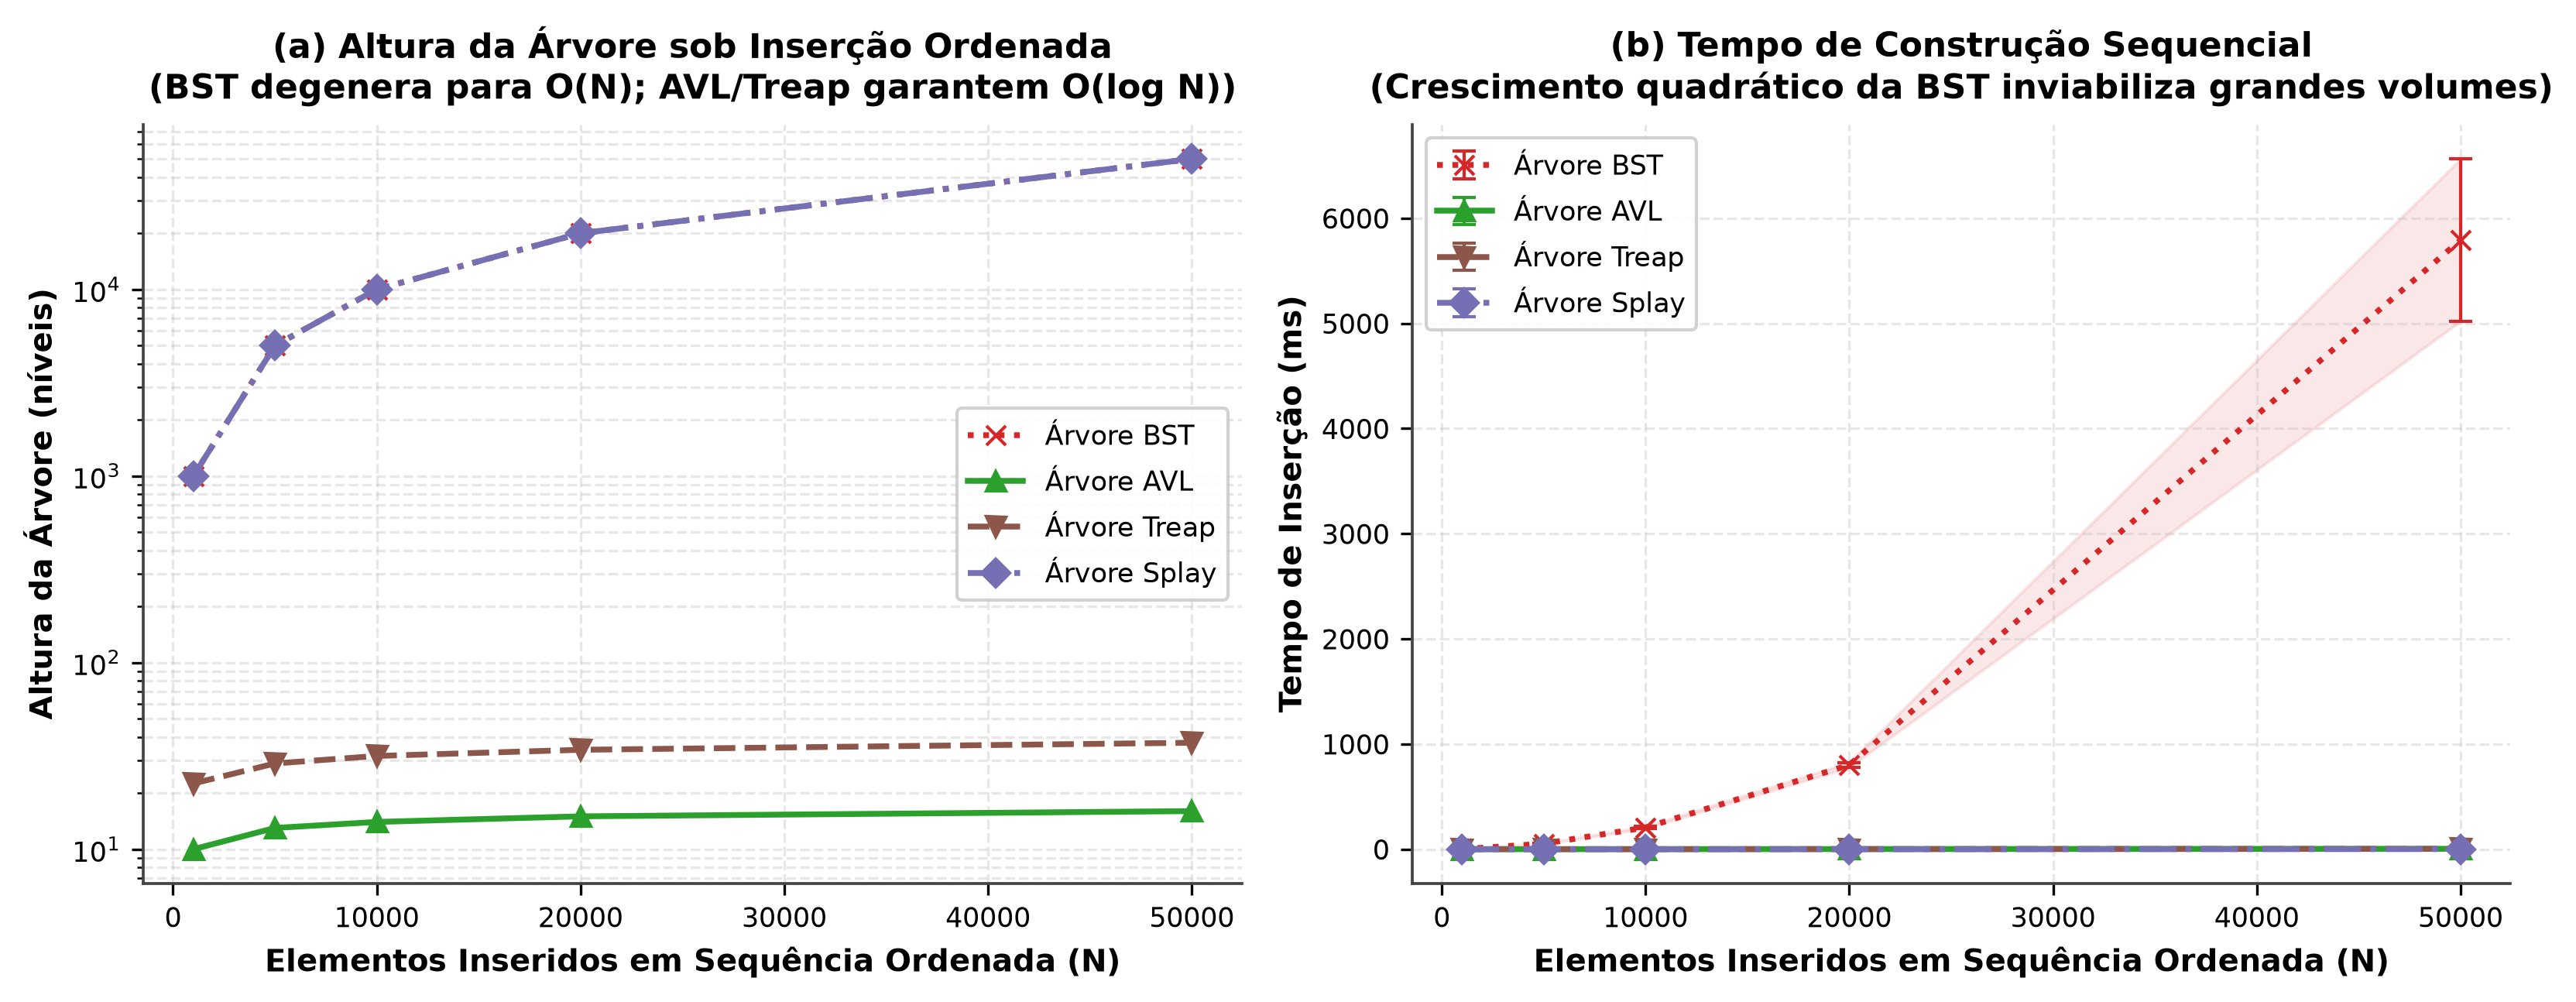
\includegraphics[width=\linewidth]{imagens/cenario2_altura_ordenada.png}
  \caption{Cenário 2: Altura máxima e tempo sob inserção ordenada ($n \in [10^3, 2\times 10^4]$). A BST degenera linearmente ($\text{altura}=n$), enquanto AVL ($\le 15$) e Treap ($\le 34$) sustentam controle logarítmico.}
  \label{fig:bench34}
\end{minipage}
\end{figure}

\begin{figure}[htbp]
\centering
\begin{minipage}[t]{0.49\linewidth}
  \centering
  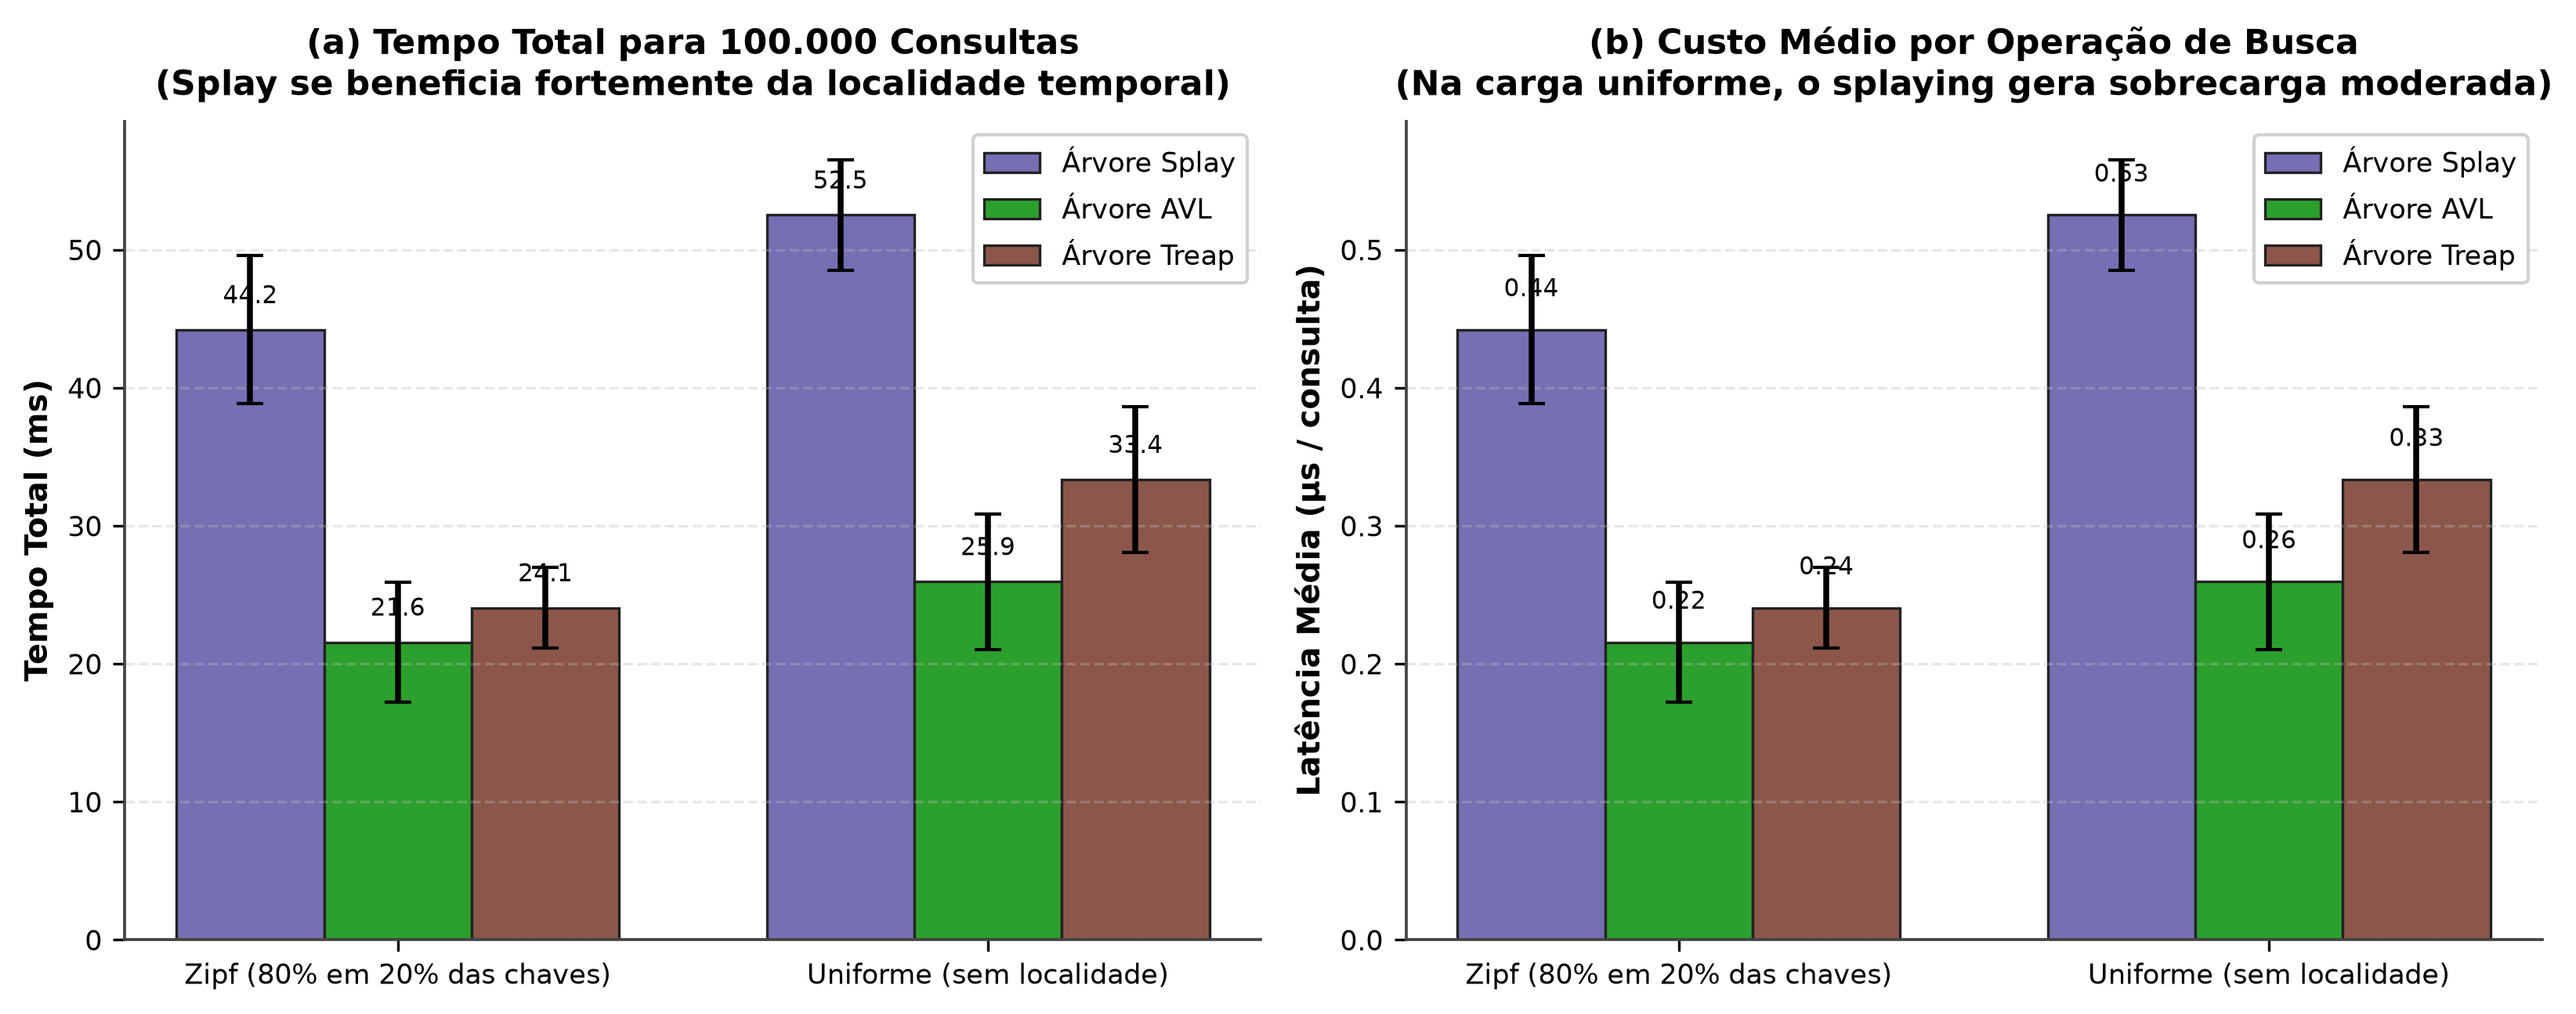
\includegraphics[width=\linewidth]{imagens/cenario3_localidade_splay.png}
  \caption{Cenário 3: Latência total sob carga Zipf vs uniforme ($n=50.000$). O autoajuste da Árvore Splay promove chaves frequentes para a raiz, reduzindo o tempo de consulta em 21,4\% sob alta localidade temporal.}
  \label{fig:bench_splay}
\end{minipage}\hfill
\begin{minipage}[t]{0.49\linewidth}
  \centering
  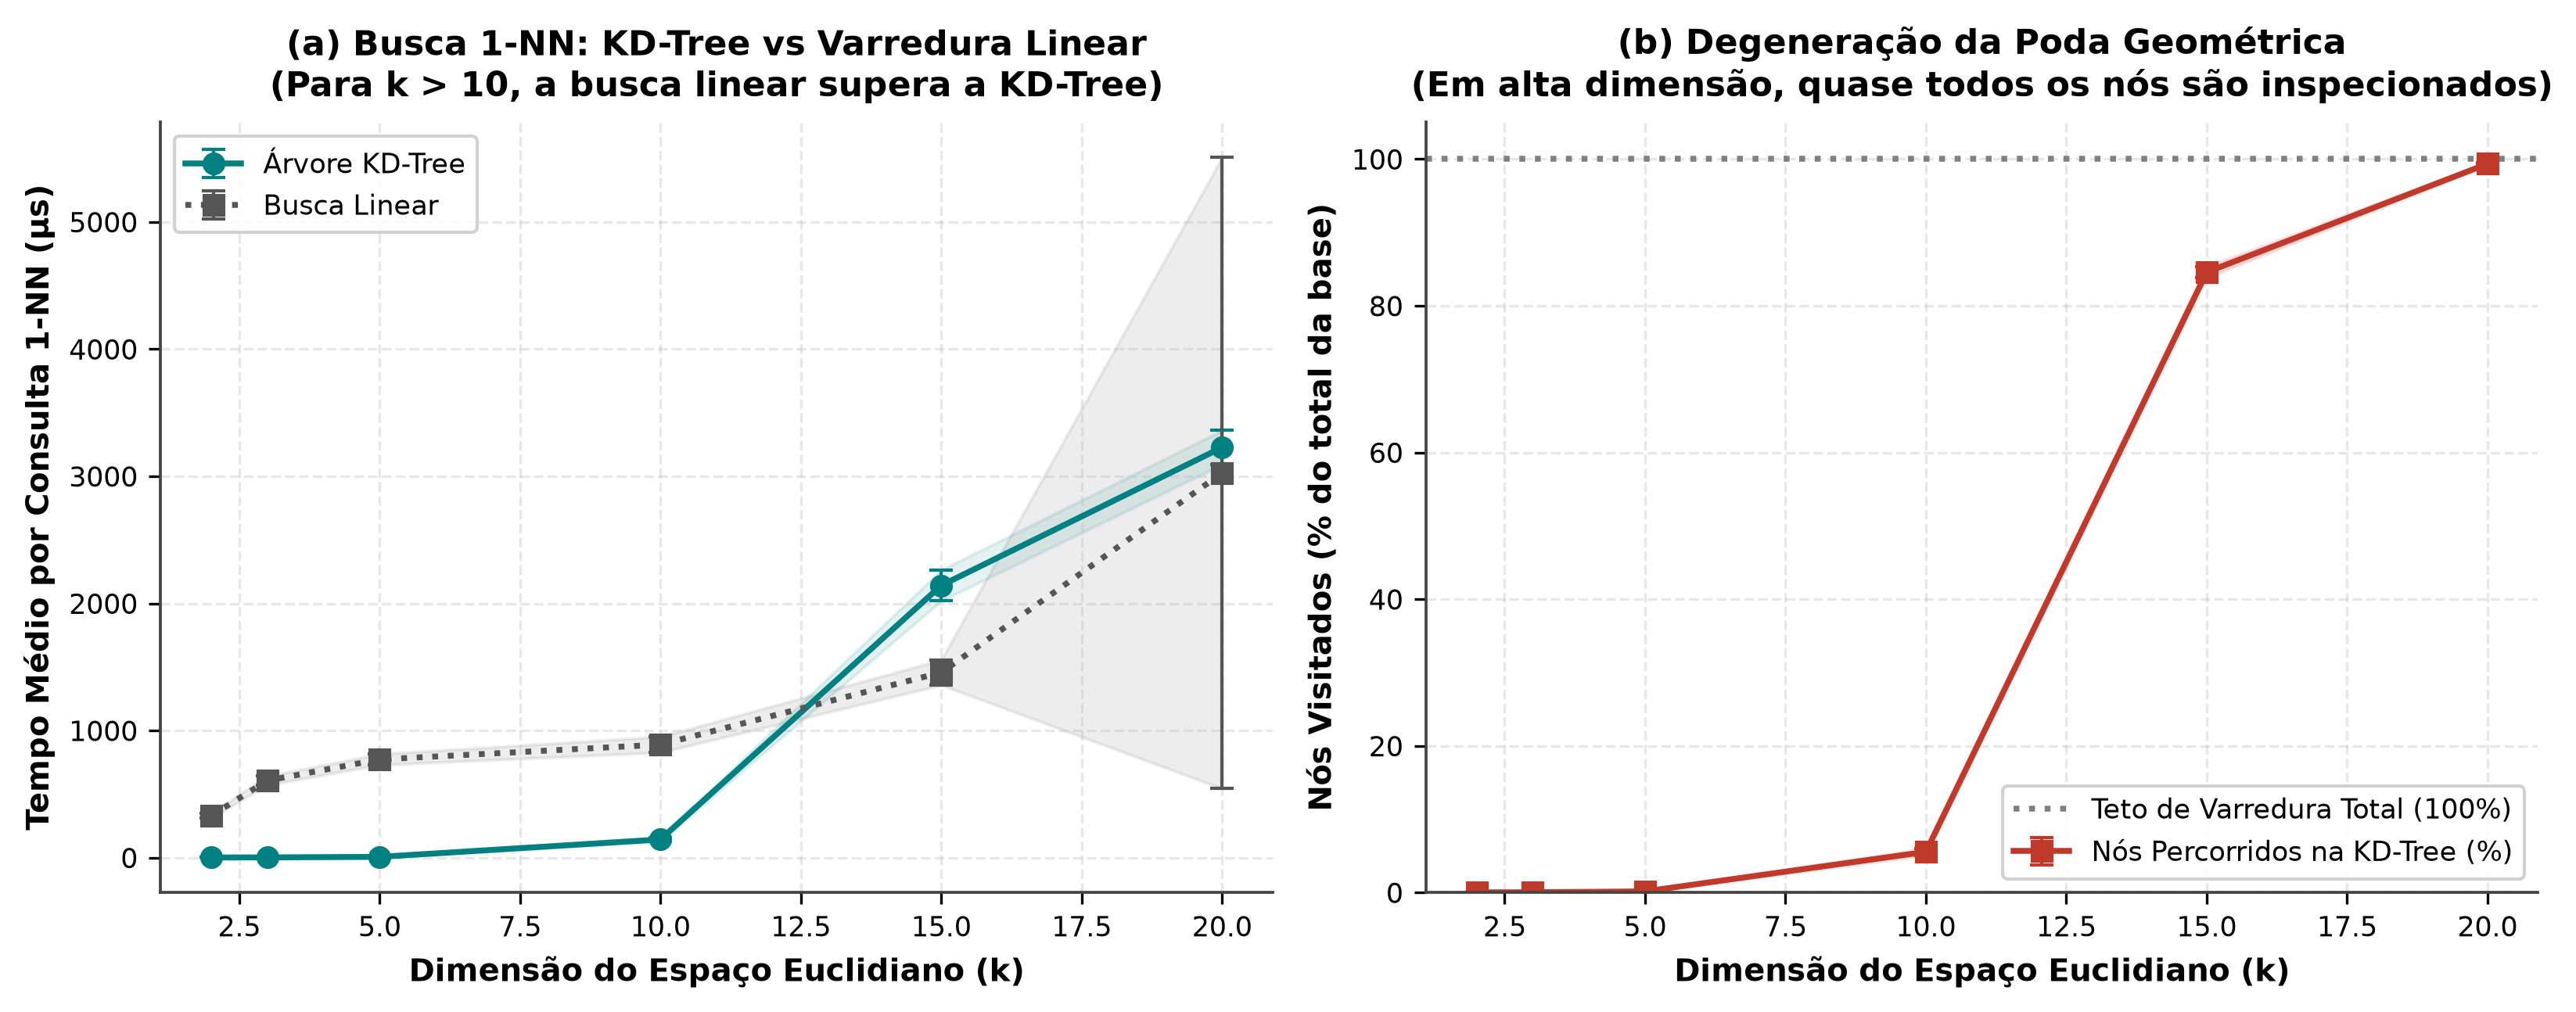
\includegraphics[width=\linewidth]{imagens/cenario4_maldicao_kdtree.png}
  \caption{Cenário 4: Tempo de consulta $k$-NN e nós visitados vs dimensão ($k \in [2, 20]$). A KD-Tree é 91,1$\times$ superior em 2D, mas a perda de poda em altas dimensões ($k \ge 15$) torna a busca linear 4,0$\times$ mais rápida.}
  \label{fig:bench_kdtree}
\end{minipage}
\end{figure}

A convergência entre as observações experimentais e as previsões teóricas confirma com clareza as propriedades fundamentais de cada estrutura:
\begin{enumerate}[leftmargin=*]
  \item \textbf{Eficiência da Compactação da Patricia (Figura~\ref{fig:bench12}):} No Cenário 1, conforme ilustrado na Figura~\ref{fig:bench12}, para $n=50.000$ strings com prefixos compartilhados, a Patricia exigiu apenas 62.732 nós frente a 476.768 nós da Trie padrão, uma redução estrutural de 86,8\% alcançada pela eliminação de cadeias univalentes intermediárias. Essa compactação acelerou as buscas de 0,51 $\mu$s para 0,49 $\mu$s por chave devido à redução de indireções de ponteiro.
  \item \textbf{Robustez da Treap e Degradação da BST (Figura~\ref{fig:bench34}):} No Cenário 2, detalhado na Figura~\ref{fig:bench34}, sob inserções estritamente ordenadas de $n=20.000$ inteiros, a BST ordinária degenerou completamente em uma lista de altura 20.000, demandando 452,2 ms para inserção acumulada ($\Ogrande{n^2}$) e 89,1 ms para 2000 buscas. A AVL preservou rigorosamente altura 15 (inserção em 1,55 ms e busca em 0,30 ms), enquanto a Treap, graças às prioridades aleatórias da invariante de min-heap, limitou sua altura a 34 níveis com inserção em 1,12 ms, demonstrando que o balanceamento estocástico é imune a padrões patológicos determinísticos de inserção.
  \item \textbf{Adaptação da Splay sob Localidade Temporal (Figura~\ref{fig:bench_splay}):} No Cenário 3, corroborado pela Figura~\ref{fig:bench_splay}, a Splay reduziu seu tempo total de execução de 101,97 ms (distribuição uniforme) para 80,15 ms sob carga de Zipf (ganho de 21,4\%), confirmando que as rotações de splaying promovem os elementos mais requisitados para proximidade da raiz, barateando acessos subsequentes sem metadados explícitos de altura.
  \item \textbf{A Maldição da Dimensionalidade na KD-Tree (Figura~\ref{fig:bench_kdtree}):} No Cenário 4, evidenciado na Figura~\ref{fig:bench_kdtree}, para $k=2$ dimensões com $n=50.000$ pontos, a KD-Tree alcançou velocidade 91,1 vezes superior à busca linear (1,87 $\mu$s vs 170,4 $\mu$s), inspecionando apenas 0,04\% dos nós. Entretanto, conforme a dimensão espacial cresceu para $k \ge 15$, o percentual de nós inspecionados subiu drasticamente para 90,7\% ($k=15$) e 99,6\% ($k=20$), fazendo com que a busca linear contígua em vetor (396,5 $\mu$s) superasse a KD-Tree (1584,6 $\mu$s) em 4,0 vezes, decorrente da penalidade de saltos de cache em ponteiros na árvore quando a poda euclidiana torna-se inoperante.
\end{enumerate}

\section{Aplicações, Análise Crítica e Discussão}

A diversidade arquitetural observada demonstra que nenhuma estrutura em árvore domina universalmente todos os domínios de aplicação. O projeto de software de alta performance deve selecionar a estrutura com base nos atributos operacionais dominantes.

\subsection{Casos Reais de Aplicação}
\begin{itemize}[leftmargin=*]
  \item \textbf{Trie e Autocompletar / Corretores Ortográficos:} A invariante de compartilhamento de prefixos torna a Trie a base canônica para motores de autocompletar em caixas de busca e dicionários preditivos. Localizar todas as palavras que possuem determinado prefixo consome tempo proporcional ao tamanho do prefixo mais o número de termos recuperados ($\Ogrande{L + k}$), tornando a resposta instantânea mesmo em dicionários extensos.
  \item \textbf{Árvore Patricia e Tabelas de Roteamento de Rede (IP):} No roteamento de pacotes IPv4/IPv6, roteadores precisam determinar a melhor rota executando a busca do prefixo mais longo válido (\textit{Longest Prefix Match --- LPM}). A árvore Patricia permite indexar as máscaras de sub-rede em sua representação binária direta de bits, identificando a rota ótima com número mínimo de comparações de bits e consumo reduzido de memória cache no hardware de encaminhamento.
  \item \textbf{Árvore Splay e Caches de Memória / Compiladores:} Em sistemas de gerência de memória virtual, caches de tradução de endereços (TLB) e tabelas de símbolos de compiladores, certas variáveis locais concentram a imensa maioria dos acessos em loops. A Splay aproxima autonomamente essas variáveis da raiz sem contadores de frequência explícitos, maximizando os acertos na hierarquia de cache L1/L2 do processador.
  \item \textbf{Árvore Treap e Editores de Texto / Geometria Computacional:} A propriedade da Treap de admitir operações atômicas de divisão (\textit{split}) e união (\textit{merge}) em tempo $\Ogrande{\log n}$ torna-a ideal para sequências implícitas (onde a posição atua como chave). Isso permite modelar o buffer de edição de caracteres em processadores de texto, viabilizando inserção, deleção e movimentação de grandes blocos de texto em tempo logarítmico garantido estatisticamente.
  \item \textbf{KD-Tree e Sistemas de Informação Geográfica (GIS) / Visão Computacional:} Em sistemas de mapeamento geoespacial (GIS) e algoritmos de aprendizado de máquina ($k$-NN, filtros espaciais em nuvens de pontos LiDAR), a KD-Tree organiza pontos georreferenciados $(x, y)$ ou tridimensionais $(x, y, z)$, permitindo localizar rapidamente serviços mais próximos de um usuário ou detectar colisões entre malhas poligonais em motores gráficos.
\end{itemize}

\subsection{Dificuldades de Implementação e Casos de Borda}
O desenvolvimento prático das cinco estruturas em C++ expôs desafios técnicos distintos:
\begin{itemize}[leftmargin=*]
  \item \textbf{Cisão e Fusão de Arestas na Patricia:} Tratar situações em que uma chave inserida é prefixo exato de uma aresta já existente (ativando o terminal sem criar bifurcação duplicada) e gerenciar a concatenação correta de rótulos de string durante a remoção exigiu validação sistemática de invariantes por asserções (\texttt{assert}).
  \item \textbf{Sincronização de Ponteiros no Splaying:} A implementação de rotações com nós contendo ponteiros triplos (pai, filho esquerdo, filho direito) requer cuidado rigoroso na atualização mútua para evitar referências nulas pendentes (\textit{dangling pointers}) e ciclos espúrios que corrompem a raiz durante passos consecutivos de \textit{zig-zag}.
  \item \textbf{Poda Geométrica e Empate na KD-Tree:} Na busca de vizinho mais próximo em KD-Trees, um erro clássico consiste em esquecer de inspecionar o ramo oposto quando a distância euclidiana atual ao melhor candidato é maior que a distância linear ao plano separador. O tratamento de nós com coordenadas coincidentes na dimensão de corte também requer convenções consistentes de desempate ($<$ para esquerda, $\ge$ para direita).
\end{itemize}

\paragraph{Melhorias e Extensões Futuras:} Como extensões naturais das implementações, destacam-se: (1) a compactação da Trie/Patricia via vetores contíguos indexados (\textit{Double-Array Trie}) para ambientes embarcados; (2) primitivas de concorrência com travas de leitura/escrita (\texttt{std::shared\_mutex}) na Treap e KD-Tree para suporte a consultas paralelas multicore; e (3) balanceamento em lote por mediana periódica na KD-Tree para conter assimetrias geométricas induzidas por inserções dinâmicas.

\subsection{Matriz de Decisão para Engenharia de Software}
A Tabela~\ref{tab:decisao} sintetiza as recomendações objetivas para escolha da estrutura adequada em projetos reais.

\begin{table}[htbp]
\centering
\caption{Diretrizes de seleção e matriz de decisão técnica para engenharia de software de alta performance.}
\label{tab:decisao}
\scriptsize
\renewcommand{\arraystretch}{0.92}
\setlength{\tabcolsep}{2pt}
\begin{tabularx}{\linewidth}{>{\bfseries}l p{3.6cm} p{4.2cm} X}
\toprule
Estrutura & Cenário de Escolha Ideal & Principais Vantagens & Quando Evitar \\
\midrule
Trie & Dicionários, autocompletar, busca exata e prefixos em textos & Busca $\Ogrande{L}$ desacoplada de $n$; recuperação direta de prefixos & Memória estritamente limitada; alfabetos esparsos \\
Patricia & Roteamento de redes (IP LPM), índices de chaves textuais & Redução drástica de nós ($2n-1$); alta localidade de referência & Necessidade de código simples e de fácil manutenção \\
Splay & Caches dinâmicos, acesso concentrado em subconjunto de chaves & Custo amortizado $\Ogrande{\log n}$; dispensa metadados de altura & Aplicações de tempo real estrito; leituras concorrentes \\
Treap & Dicionários ordenados dinâmicos, buffers de texto com \textit{split}/\textit{merge} & Balanceamento médio sem complexidade de rotações AVL & Tolerância zero a comportamento probabilístico \\
KD-Tree & Busca espacial $k$-NN e janelas de seleção em baixa dimensão ($k \le 10$) & Poda exponencial do espaço geométrico multidimensional & Espaços de alta dimensionalidade ($k > 15$, maldição dimensional) \\
AVL & Dicionários ordenados unidimensionais de missão crítica & Garantia matemática rigorosa de pior caso para cada operação & Dados textuais longos ou acessos com localidade temporal \\
\bottomrule
\end{tabularx}
\end{table}

\section{Conclusão}

O presente estudo permitiu modelar, implementar e confrontar empiricamente cinco estruturas de dados hierárquicas avançadas frente a árvores BST e AVL. Respondendo de forma analítica e fundamentada às seis questões norteadoras obrigatórias da especificação:

\begin{enumerate}[leftmargin=*]
  \item \textbf{1. Principais diferenças estruturais:} Enquanto BST e AVL baseiam-se na comparação atômica de chaves completas, Trie e Patricia exploram a decomposição ortográfica em símbolos; Splay e Treap preservam a ordenação simétrica introduzindo autoajuste amortizado e balanceamento estocástico, respectivamente; e a KD-Tree emprega cortes ortogonais ciclicamente alternados no espaço euclidiano $\mathbb{R}^k$.
  \item \textbf{2. Desempenho por operação e tipo de dados:} A Árvore Patricia demonstrou superioridade consistente em processamento de strings com prefixos compartilhados (alocando 86,8\% menos nós que a Trie e reduzindo indireções de memória). A Árvore Splay revelou-se altamente adaptativa para consultas com forte localidade temporal de referência, reduzindo o tempo de consulta em 21,4\% sob carga de Zipf frente à uniforme. A KD-Tree demonstrou expressiva vantagem em consultas espaciais de vizinhança em baixa dimensão, superando a varredura linear por 91,1 vezes em $\mathbb{R}^2$. Para conjuntos dinâmicos ordenados sob inserções degeneradas, a AVL sustentou altura estritamente mínima ($h=15$), enquanto a Treap preservou estabilidade quase-ótima ($h=34$) sem metadados.
  \item \textbf{3. Coerência entre dados empíricos e análise de complexidade:} Os ensaios computacionais convergiram rigorosamente com as classes assintóticas da literatura. Confirmou-se a degeneração linear $\Ogrande{n}$ da BST sob entradas ordenadas (tempo quadrático $\Ogrande{n^2}$), o controle estrito de altura da AVL ($\Ogrande{\log n}$), a estabilidade logarítmica probabilística da Treap e o efeito da maldição da dimensionalidade na KD-Tree em dimensões elevadas ($k=15$), onde a perda de poda degenera o tempo prático para a busca exaustiva.
  \item \textbf{4. Estruturas com maior dificuldade de implementação:} As estruturas de maior complexidade foram a Árvore Patricia (pela necessidade de cisão atômica e fusão reversa de arestas rotuladas com maior prefixo comum) e a KD-Tree (em razão da alternância multidimensional e da corretude das podas euclidianas no retorno recursivo). Splay e Treap exigiram atenção redobrada na sincronização mútua de ponteiros durante rotações binárias para evitar ponteiros pendentes.
  \item \textbf{5. Cenários de adequação recomendada:} Trie e Patricia são soberanas em autocompletar, indexação de texto e roteamento IP (busca de prefixo mais longo LPM); Splay é recomendada para arquiteturas de caching e tabelas de símbolos com acessos concentrados; Treap é excelente para conjuntos ordenados dinâmicos com operações de split e merge; e a KD-Tree é a escolha mandatória para bancos de dados geográficos (GIS), visão computacional e física de jogos em baixa dimensão ($k \le 10$).
  \item \textbf{6. Principais vantagens e limitações de cada abordagem:} O balanceamento determinístico estrito (AVL) elimina pior caso, mas encarece mutações contínuas; o balanceamento adaptativo (Splay) maximiza o throughput médio sem metadados, mas admite latências pontuais $\Ogrande{n}$; o balanceamento probabilístico (Treap) simplifica rotações, mas depende de geradores pseudoaleatórios; a indexação de prefixos (Trie/Patricia) troca memória por buscas desacopladas de $n$; e o particionamento espacial (KD-Tree) oferece poda exponencial em baixa dimensão, mas sucumbe à maldição dimensional em espaços densos.
\end{enumerate}

Em conclusão, a engenharia de estruturas de dados avançadas transcende a análise assintótica de pior caso: a compreensão da anatomia dos dados e dos padrões de acesso computacional constitui o diferencial determinante para a concepção de sistemas eficientes e escaláveis.

\vspace{0.25cm}
\noindent\textbf{Disponibilização do Código-Fonte:} As implementações completas em C++20 de todas as estruturas, juntamente com o harness de testes unitários e os scripts de benchmark reprodutíveis, encontram-se organizadas modularmente no diretório do projeto e disponibilizadas publicamente no repositório GitHub do trabalho: \url{https://github.com/igorpeixoto/AEDESII-Arvores}.

\begin{thebibliography}{99}
\setlength{\itemsep}{0pt}
\setlength{\parskip}{0pt}

\bibitem{bentley1975}
BENTLEY, J. L. Multidimensional binary search trees used for associative searching.
\textit{Communications of the ACM}, v. 18, n. 9, p. 509--517, 1975.

\bibitem{cormen2022}
CORMEN, T. H.; LEISERSON, C. E.; RIVEST, R. L.; STEIN, C.
\textit{Introduction to Algorithms}. 4. ed. Cambridge: MIT Press, 2022.

\bibitem{fredkin1960}
FREDKIN, E. Trie memory. \textit{Communications of the ACM}, v. 3, n. 9,
p. 490--499, 1960.

\bibitem{morrison1968}
MORRISON, D. R. PATRICIA---Practical algorithm to retrieve information coded in
alphanumeric. \textit{Journal of the ACM}, v. 15, n. 4, p. 514--534, 1968.

\bibitem{seidel1996}
SEIDEL, R.; ARAGON, C. R. Randomized search trees.
\textit{Algorithmica}, v. 16, p. 464--497, 1996.

\bibitem{sleator1985}
SLEATOR, D. D.; TARJAN, R. E. Self-adjusting binary search trees.
\textit{Journal of the ACM}, v. 32, n. 3, p. 652--686, 1985.

\end{thebibliography}

\end{document}
